\documentclass{beamer}
\usepackage[utf8]{inputenc}

\usetheme{Madrid}
\usecolortheme{default}
\usepackage{amsmath,amssymb,amsfonts,amsthm}
\usepackage{txfonts}
\usepackage{tkz-euclide}
\usepackage{listings}
\usepackage{adjustbox}
\usepackage{array}
\usepackage{tabularx}
\usepackage{gvv}
\usepackage{lmodern}
\usepackage{circuitikz}
\usepackage{tikz}
\usepackage{graphicx}
\usepackage[T1]{fontenc}
\usepackage[utf8]{inputenc}

\lstset{
  language=Python,
  basicstyle=\ttfamily\small,
  breaklines=true,
  literate={λ}{{$\lambda$}}1
}



\setbeamertemplate{page number in head/foot}[totalframenumber]

\usepackage{tcolorbox}
\tcbuselibrary{minted,breakable,xparse,skins}



\definecolor{bg}{gray}{0.95}
\DeclareTCBListing{mintedbox}{O{}m!O{}}{%
  breakable=true,
  listing engine=minted,
  listing only,
  minted language=#2,
  minted style=default,
  minted options={%
    linenos,
    gobble=0,
    breaklines=true,
    breakafter=,,
    fontsize=\small,
    numbersep=8pt,
    #1},
  boxsep=0pt,
  left skip=0pt,
  right skip=0pt,
  left=25pt,
  right=0pt,
  top=3pt,
  bottom=3pt,
  arc=5pt,
  leftrule=0pt,
  rightrule=0pt,
  bottomrule=2pt,
  toprule=2pt,
  colback=bg,
  colframe=orange!70,
  enhanced,
  overlay={%
    \begin{tcbclipinterior}
    \fill[orange!20!white] (frame.south west) rectangle ([xshift=20pt]frame.north west);
    \end{tcbclipinterior}},
  #3,
}
\lstset{
    language=C,
    basicstyle=\ttfamily\small,
    keywordstyle=\color{blue},
    stringstyle=\color{orange},
    commentstyle=\color{green!60!black},
    numbers=left,
    numberstyle=\tiny\color{gray},
    breaklines=true,
    showstringspaces=false,
}
\begin{document}

\title 
{4.2.18}
\date{September 29,2025}


\author 
{Bhoomika V - EE25BTECH11015}




\frame{\titlepage}
\begin{frame}{Question}
Find the direction and normal vectors of each of the following line $y = x - 2$ \\ \\ 
\end{frame}

\begin{frame}{Solution}
\begin{equation}
y = x - 2
\tag{4.2.18.1}
\end{equation}

\[
\Rightarrow
\begin{pmatrix}
x \\ y
\end{pmatrix}
=
\begin{pmatrix}
x \\ x-2
\end{pmatrix}
=
\begin{pmatrix}
0 \\ -2
\end{pmatrix}
+ x
\begin{pmatrix}
1 \\ 1
\end{pmatrix}
\tag{4.2.18.2}
\]
\end{frame}

\begin{frame}{Direction Vector}
yielding
\begin{equation}
\vec{x} = \vec{h} + \kappa \vec{m}
\tag{4.2.18.3}
\end{equation}

where $\vec{h}$ is any point on the line and  

\[
\vec{m} =
\begin{pmatrix}
1 \\ 1
\end{pmatrix}
\tag{4.2.18.4}
\]

is the direction vector.  

\end{frame}

\begin{frame}{Normal Vector}
\subsection*{4.1.2 For normal vector}

\begin{equation}
\vec{m}^T \vec{n} = 0
\tag{4.2.18.5}
\end{equation}

\[
\vec{n}^T \vec{x} = \vec{n}^T \vec{h} + \kappa \vec{n}^T \vec{m}
\tag{4.2.18.6}
\]

\[
\Rightarrow \vec{n}^T (\vec{x} - \vec{h}) = 0
\quad \text{or} \quad
\vec{n}^T \vec{x} = c
\tag{4.2.18.7}
\]

for
\begin{equation}
c = \vec{n}^T \vec{h}
\tag{4.2.18.8}
\end{equation}
\end{frame} 

\begin{frame}{}
where
\[
\vec{n} =
\begin{pmatrix}
-m \\ 1
\end{pmatrix}
\tag{4.2.18.9}
\]

\[
\begin{pmatrix}
-1 \\ 1
\end{pmatrix}
\]




is defined to be the \textit{normal vector} of the line.
\end{frame} 

\begin{frame}[fragile]
    \frametitle{C Code - A function to find if triangle is right angled }

    \begin{lstlisting}
#include <stdio.h>

// Function to compute direction and normal vectors for a line y = x - 2
// General form: x - y - 2 = 0
// Normal vector = (a, b) = (1, -1)
// Direction vector = (b, -a) = (-1, -1)

void line_vectors(float *dx, float *dy, float *nx, float *ny) {
    float a = 1, b = -1;   // coefficients of x - y - 2 = 0

    // Normal vector
    *nx = a;
    *ny = b;

    // Direction vector
    *dx = b;
    *dy = -a;
}
     \end{lstlisting}
\end{frame}

\begin{frame}[fragile]
    \frametitle{Python Code}
    \begin{lstlisting}
import numpy as np
import matplotlib.pyplot as plt
import ctypes   #included

# --- Load the C library ---
try:
    c_lib = ctypes.CDLL('./line.so')
except OSError:
    print(" Error: 'line.so' not found. Compile using: gcc -shared -o line.so -fPIC line_vectors.c")
    exit()

# Define argument and return types
c_lib.line_vectors.argtypes = [ctypes.POINTER(ctypes.c_float),
                               ctypes.POINTER(ctypes.c_float),
                               ctypes.POINTER(ctypes.c_float),
                               ctypes.POINTER(ctypes.c_float)]
c_lib.line_vectors.restype = None
        \end{lstlisting}
\end{frame}

\begin{frame}[fragile]
    \frametitle{Python Code}
    \begin{lstlisting}
# --- Prepare ctypes variables ---
dx = ctypes.c_float()
dy = ctypes.c_float()
nx = ctypes.c_float()
ny = ctypes.c_float()

# --- Call C function ---
c_lib.line_vectors(ctypes.byref(dx), ctypes.byref(dy), ctypes.byref(nx), ctypes.byref(ny))

print(f" Direction vector: ({dx.value}, {dy.value})")
print(f" Normal vector: ({nx.value}, {ny.value})")

# --- Plot the line y = x - 2 ---
x = np.linspace(-2, 6, 100)
y = x - 2
fig, ax = plt.subplots()
ax.plot(x, y, label="Line: y = x - 2", color="black")

# --- Choose a point on the line ---
P = np.array([2, 0], dtype=float)
        \end{lstlisting}
\end{frame}

\begin{frame}[fragile]
    \frametitle{Python Code}
    \begin{lstlisting}


# Plot direction vector
ax.arrow(P[0], P[1], dx.value, dy.value, 
         head_width=0.2, color="red", length_includes_head=True, label="Direction Vector")

# Plot normal vector
ax.arrow(P[0], P[1], nx.value, ny.value, 
         head_width=0.2, color="blue", length_includes_head=True, label="Normal Vector")

# Formatting
ax.set_xlabel("X-axis")
ax.set_ylabel("Y-axis")
ax.set_title("Line y = x - 2 with Direction & Normal Vectors")
ax.legend()
ax.grid(True)
ax.set_aspect("equal")

plt.show()
        \end{lstlisting}
\end{frame}


\begin{frame}{Plot}
    \centering
    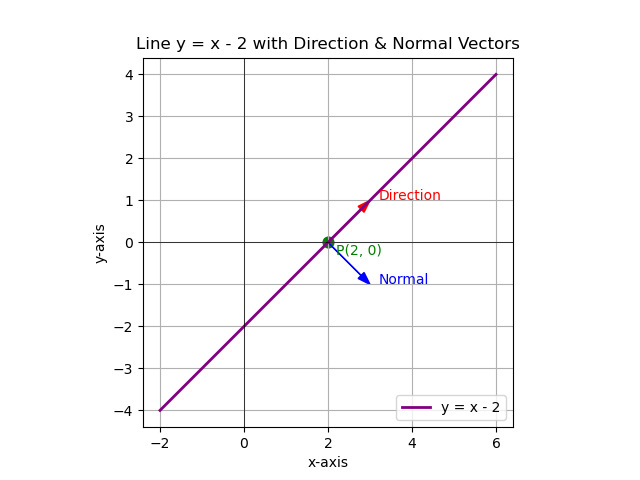
\includegraphics[width=\columnwidth, height=0.8\textheight, keepaspectratio]{Figs/Fig1.png}     
\end{frame}



\end{document}